\chapter{Multiset Rewriting and P Systems}
A formal specification of chemical reaction and of their behavior can be given in terms of \textbf{MultiSet Rewriting (MSR)}.\par

\section{Multiset}
With \textbf{multiset} we intend a variant of the mathematical notion of set in which elements can be repeated. In this way we can interpret chemical solution as multisets representing molecules.

\subsection{Formalizing multisets}
Given a (finite or infinite) support set $\Sigma$, we methematically represent a multiset M over $\Sigma$ in two ways:
\begin{itemize}
    \item \textbf{set of pairs:} $M \subseteq \Sigma \times \mathbb{N}$
    \item \textbf{ mapping:} $M: \Sigma \rightarrow \mathbb{N}$
\end{itemize}

\subsubsection{Example}
Given the set $\Sigma = \{A, B, C\}$ and the multiset $M = \{A, A, A, B, B, C, C, C \}$ over $\Sigma$ can be represented in two ways:

\begin{itemize}
    \item \textbf{set of pairs:} $M = \{ (A, 3), (B, 2), (C, 3) \}$
    \item \textbf{mapping:} $M(A) = 3, M(B) = 2, M(C) = 3$
\end{itemize}

\textbf{Note:} these representations actually correspond to the representation of chemical solutions we considered in PRISM.

\subsection{Representing Multisets as strings}
Another useful representation of multisets that is very similar to formal grammars is a \textbf{string}.\par
We interpret the set $\Sigma$ as an \textbf{alphabet}, and the multiset $M$ over $\Sigma$ correspond to strings over such alphabet. Note that in a string representing a multiset, \textbf{the order of the symbols does not matter}, so string permutations result in equivalent representation.

\subsubsection{Example}
Given $\Sigma = \{A, B, C\}$ and the multiset $M = \{(A, 3), (B,2), (C,3)\}$ we can represent M as the string:
$M = AAABBCCC = A^{3}B^{2}C^{3}$ and all its possible permutations.\par
Multiset union can be expressed as string concatenation:
\begin{equation*}
\{(A,3), (B,2), (C,3) \} \cup \{ (A,2), (B,1)\} = \{(A,5), (B,3), (C,3)\} = A^{5}B^{3}C{3}    
\end{equation*}

\section{Representing reactions as rewriting rules}
Rules are similar to rules in a formal grammar:\par
A multiset rewriting rule is a pair $(u, v)$ with $u, v \in \Sigma^{*}$ usually denoted as $\mapsto$. When we apply the rule $(u,v)$ to a multiset $w \in \Sigma^{*}$ s.t. $u \subseteq w$ what we obtain is the multiset in which \textbf{$u$ as been replaced by $v$}

\section{Definition of MultiSet Rewriting System}
A MultiSet Rewriting System (MSRS) is a pair $S = < \Sigma, \mathcal{R} >$ where $\Sigma$ is the \textbf{alphabet of symbols} and  $\mathcal{R}$ is a \textbf{set of multiset rewriting rules}.\par
Given a multiset in $\Sigma^{*}$ we can use the mechanism of rewriting rule application to compute \textbf{traces} of the multiset rewriting system.

\section{Interleaving semantics}
The behavior of a MSR system can also be described as a Transition System: we can define an (interleaving) semantics for MSR defining inference rules incorporating the mechanism of rewriting rule application.\par
The interleaving semantics of a MSR system $< \Sigma, \mathcal{R}>$ is the Transition System ${\Sigma^{*}, \rightarrow}$ where $\rightarrow \subseteq \Sigma^{*} \times \Sigma^{*}$ is the least transition relation satisfying the following inference rule:
\begin{equation*}
    \frac{u \mapsto v \in \mathcal{R}}{uw \mapsto vw}
\end{equation*}

\section{Stochastic MSR}
We can extend the stochastic syntax and semantics of MSR to incorporate stochastic rates.\par
Given an alphabet $\Sigma$ a stochastic multiset rewriting rule is a tuple $(u, v, r)$ where $u, v \in \Sigma^{*}$ and $r \in \mathbb{R}^{+}$, usually denoted $u \mapsto^{r} v$

\subsubsection{Stochastic Multiset Rewriting System}
A Stochastic MSR system is a pair $S = <\Sigma, \mathcal{R}>$ where $\Sigma$ is an alphabet of symbols and $\mathcal{R}$ is a set of stochastic multiset rewriting rules.

\subsubsection{Semantics of Stochastic MSR}
The semantics of a stochastic MSR system is a Continuous Time Markov Chain $(\Sigma^{*}, \rightarrow)$ where $\rightarrow \subseteq \sum^{*} \times \mathbb{R}^{+} \times \sigma^{*}$ is the least stochastic transition relation satisfying the following inference rule:
\begin{equation*}
    \frac{ u \mapsto^{r} v \in \mathcal{R}}{uw \xrightarrow{r \cdot f(u, uw)} vw}
\end{equation*}

Where $f(u, uw)$ gives the number of instances of $u$ in $uw$.

\section{Introducing parallelism}
We can defines variantas of the language, in particular regarding the introduction if prarallelism in the application of rewriting rules:
\begin{itemize}
    \item \textbf{simple parallelism:} one or more rule are applied at each step.
    \item \textbf{maximal parallelism:} as many rules as possible are applied at each step.
\end{itemize}
In this way we can model classes of systems where there are simultaneous events. In particular we are interested in maximal parallelism because its models system where there is a strong formal synchronization.

\subsection{Parallel semantics of MSR}
The parallel semantics of a MSR system $<\Sigma, \mathcal{R}>$ is the transition system $(\Sigma^{*}, \rightarrow)$ where $\rightarrow \subseteq \sum^{*} \times \sum^{*}$ is the lest transition relation satisfying the following inference rules:

\begin{equation*}
    \frac{u \mapsto v \in \mathcal{R}}{u \rightarrow v}
\end{equation*}

\begin{equation*}
    \frac{w_{1} \rightarrow w^{'}_{1} \ \ \ w_{2} \rightarrow w^{'}_{2}}{w_{1}w_{2} \rightarrow w^{'}_{1}w^{'}_{2}} 
\end{equation*}

\begin{equation*}
    \frac{w \rightarrow w^{'} \ \ \ u \nrightarrow}{wu \Rightarrow w^{'}{u}} 
\end{equation*}

\section{Multiset languages}
A language where we ignore the sequential ordering of symbols in its words becomes a \textbf{multiset language}. A multiset language is a set of multisets of terminal symbols and is generated by a multiset grammar.\par
This change in the representation of the language causes a significant change in the expressiveness of the languages, becoming more weak. Multiset languages can run on a weak-Turing Machine.

\subsection{Introducing maximal parallelism in multiset languages}
The maximal parallelism re-introduce the expressive power of grammars I lost using multiset languages. General multiset grammar rules applied with maximal parallelism are again able to generate any recursively enumerable language. Having a more complex grammar requires a Turing-complete form of automaton to accept a string from it.

\section{P Systems}
P Systems is a variant of Multiset rewriting with maximal parallelism (P stands for Paul which is the name of the inventor). What set apart P Systems from normal Multiset rewriting is that it has more than one multiset in the set.\par
The key elements of P Systems are:
\begin{itemize}
    \item \textbf{Membranes:} they creates compartments used to distribute computations.
    \item \textbf{Multisets:} abstraction of chemical solutions that are used as data.
    \item \textbf{Evolution (rewriting) rules:} abstraction of chemical reaction that are used as programs.
\end{itemize}

\begin{figure}[h]
    \centering
    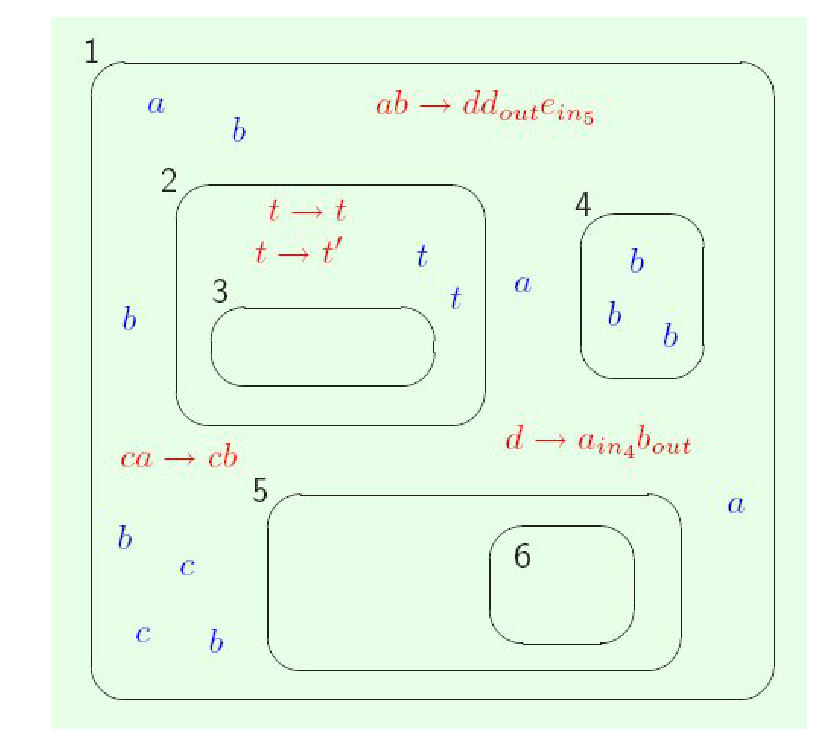
\includegraphics[width=0.5\textwidth]{Images/11-Multiset Rewriting and P Systems/PSystem.png}
    \caption{Example of a P System} 
\end{figure}

\subsection{Formal definition of a P System}
A P System $\Pi$ is given by:
\begin{equation*}
    \Pi = (V, \mu, w_{1}, ..., w_{n}, R_{1}, ..., R_{n})
\end{equation*}

where:
\begin{itemize}
    \item \textbf{V:} is an alphabet whose elements are called objects.
    \item $\mu \subset \mathbb{N} \times \mathbb{N}$ is a membrane structure, s.t. $(i, j) \in \mu$ denotes that the membrane labeled by $j$ is contained in the membrane labeled by $i$.
    \item $w_{i}$ with $1 \leq i \leq n$ are strings from $V^{*}$ representing multisets over V associated with the membranes $1, 2, ..., n$ of $\mu$.
    \item $R_i$ with $1 \leq i \leq n$ are finite sets of evolution rules associated with the membranes $1, 2, ..., n$ of $\mu$.
\end{itemize}

\subsection{Evolution rules}
An evolution rule in the form $u \rightarrow v$ consists of a multiset of objects $u$ (representing reactants) and a multised of messages $v$ (representing products). A message may have one of the following forms:
\begin{itemize}
    \item $a_{here}$: means that object $a$ remains in the same membrane. Often we omit $here$ and just leave $a$ alone.
    \item $a_{out}$: means that object $a$ is sent out of the membrane.
    \item $a_{in}$: means that object $a$ is sent into the child membrane I.
\end{itemize}

Evolution rules are classified in two ways:
\begin{itemize}
    \item \textbf{non-cooperative rules:} the left-hand side consists of a single object (e.g. $a \rightarrow b^{2}d_{out}$)
    \item \textbf{cooperative rules:} the left-hand side can be any multiset of objects (e.g. $a^{2}b \rightarrow b^{2}d_{out}$). A particular case of cooperative rules are catalytic rules, namely rules of the form $ca \rightarrow cb^{2}$ where $c$ belongs to a special set of objects called catalyst.
\end{itemize}

\subsection{Downsides of P Systems}
Programming P Systems is very difficult since evolution rules are very basic.\par
For this reason over the years have been proposed variants of P Systems, obtained by considering different types of evolution rules:
\begin{itemize}
    \item with rule priorities.
    \item with promotes and inhibitors.
    \item with dissolution of membranes.
    \item symport/antiport rules.
    \item with active membranes 
    \item and so on...
\end{itemize}